\documentclass[serif,mathserif]{beamer}
\usepackage[T1]{fontenc}
\usepackage[utf8]{inputenc}
\usepackage{amsmath, amsfonts, epsfig, xspace}
\usepackage{algorithm,algorithmic}
\usepackage{pstricks,pst-node}
\usepackage{multimedia}
\usepackage{listings}
\usepackage[normal,tight,center]{subfigure}
\setlength{\subfigcapskip}{-.5em}
\usepackage{beamerthemesplit}
\usetheme{lankton-keynote}
\usepackage{inconsolata}

\lstset{ %
  %backgroundcolor=\color{white},
  basicstyle=\footnotesize\ttfamily,
  breakatwhitespace=false,
  %breaklines=true,
  captionpos=b,
  %commentstyle=\color{mygreen},
  escapeinside={\%*}{*)},
  extendedchars=true,
  %frame=single,
  %keywordstyle=\color{blue},
  %numbers=left,
  %numbersep=5pt,
  %numberstyle=\tiny\color{mygray},
  %rulecolor=\color{black},
  %showspaces=false,
  %showstringspaces=false,
  %showtabs=false,
  stepnumber=2,
  %stringstyle=\color{mymauve},
  %tabsize=2,
  %title=\lstname,
  morekeywords={external},
}

\author{Frédéric Bour}

\title[Cuite\hspace{2em}\insertframenumber/\inserttotalframenumber]{Cuite: Qt 5 bindings for OCaml}

\date{November 8, 2017}

%\institute{Justice League of America}

\begin{document}

\maketitle

\section{Qt?} 

\begin{frame}
  \frametitle{Qt?}
  \begin{itemize}
  \item A C++ framework for Desktop and Mobile apps\pause
  \item Abstracting "platforms": \\
    (stdlib, {\bf windowing system}, {\bf GUI}, VFS, networking, "XML", \ldots)\pause
  \item Cross-platform: \\
    Linux (X11, Wayland, Android), macOS, iOS, Windows, Blackberry, Sailfish OS, \ldots
  \end{itemize}
\end{frame}

\begin{frame}
  \frametitle{Used by KDE}
  \includegraphics[width=\textwidth]{apps_kde}
\end{frame}

\begin{frame}
  \frametitle{Google Earth}
  %\includegraphics[height=\textheight,width=\textwidth]{apps_kde}
  \includegraphics[height=0.9\textheight]{apps_earth}
\end{frame}

\begin{frame}
  \frametitle{Adobe Photoshop Elements}
  %\includegraphics[height=\textheight,width=\textwidth]{apps_kde}
  \includegraphics[width=\textwidth]{apps_photoshop}
\end{frame}

\begin{frame}
  \frametitle{AMD Code XL}
  %\includegraphics[height=\textheight,width=\textwidth]{apps_kde}
  \includegraphics[width=\textwidth]{apps_codexl}
\end{frame}

\begin{frame}
  \frametitle{Musescore (Desktop)}
  %\includegraphics[height=\textheight,width=\textwidth]{apps_kde}
  \includegraphics[width=\textwidth]{apps_musescore}
\end{frame}

\begin{frame}
  \frametitle{Musescore (iOS)}
  \center
  \includegraphics[height=0.9\textheight]{apps_musescore_ios}
\end{frame}

\begin{frame}
  \frametitle{Musescore (Android)}
  %\includegraphics[height=\textheight,width=\textwidth]{apps_kde}
  \includegraphics[width=\textwidth]{apps_musescore_android}
\end{frame}

\begin{frame}
  \frametitle{And much more\ldots}
  Autodesk Maya, DAZ Studio, LightWave 3D, Skype, \ldots
  \bigskip

  Find out on \href{https://showroom.qt.io/}{https://showroom.qt.io/}. \pause
  \bigskip

  Now, a small demo of OCaml port.
  \pause
  Well no.

\end{frame}

\begin{frame}
  \includegraphics[width=\textwidth]{address_main}
\end{frame}

\begin{frame}
  \includegraphics[width=\textwidth]{address_edit}
\end{frame}

\begin{frame}
  \includegraphics[width=\textwidth]{address_dialog}
\end{frame}

\begin{frame}
  \includegraphics[width=\textwidth]{syntaxhl}
\end{frame}



\section{Cuite design}

\subsection{Data representation}

\begin{frame}
  \frametitle{Mapping Qt concepts to OCaml}

  Qt concepts for data representation:
  \begin{itemize}
    \item plain types (QString, int, float, \ldots)
    \item enumerations and flags
    \item object hierarchies and QObjects
    \item QVariants
  \end{itemize}
\end{frame}

\begin{frame}[fragile]
  \frametitle{Plain types}

  \begin{itemize}
    \item Don't affect memory graph
    \item Are pure values (physical identity irrelevant)
    \item Mapped to a concrete OCaml type: \\
      \begin{lstlisting}[language=C++]
        void bla(const QString& str);
      \end{lstlisting}
      \vspace{-0.4cm}
      \begin{lstlisting}[language=Caml,morekeywords={val}]
        val bla : string -> unit
      \end{lstlisting}

    \item Or to an abstract type \& a set of functions:
      \begin{lstlisting}[language=Caml,morekeywords={val}]
        val QModelIndex.row : qModelIndex qt -> int
      \end{lstlisting}
  \end{itemize}

\end{frame}

\begin{frame}[fragile]
  \frametitle{Enumeration}

  Enumeration are directly mapped to a polymorphic variant.
  \begin{lstlisting}[language=C++]
  enum QStandardPaths::LocationOption {
    LocateFile,
    LocateDirectory
  };
  \end{lstlisting}

  \begin{lstlisting}[language=Caml]
  type qStandardPaths'LocationOption = [
    | `LocateFile
    | `LocateDirectory
    | `Invalid_value of int
  ]
  \end{lstlisting}
\end{frame}

\begin{frame}[fragile]
  \frametitle{Flags}

  Flags are unions of elements from an enumeration.  They are manipulated with
  a generic module and a witness for each flag type.

  \begin{lstlisting}[language=Caml,morekeywords={val}]

  type 'flag set
  val define : ('flag -> int64) -> 'flag set
  
  type 'flag t = private int64
  val empty : _ t
  val set : 'flag set -> 'flag -> 'flag t -> 'flag t
  val is_set : 'flag set -> 'flag -> 'flag t -> bool

  ...
  \end{lstlisting}
\end{frame}

\begin{frame}[fragile]
  \frametitle{Flags}

  Flags are unions of elements from an enumeration.  They are manipulated with
  a generic module and a witness for each flag type.

  \begin{lstlisting}[language=Caml,morekeywords={val}]

  type 'flag set
  val define : ('flag -> int64) -> 'flag set
  
  type 'flag t = private int64
  val empty : _ t
  val set : 'flag set -> 'flag -> 'flag t -> 'flag t
  val is_set : 'flag set -> 'flag -> 'flag t -> bool

  ...
  \end{lstlisting}
\end{frame}

\begin{frame}
  \frametitle{Object hierarchy}

  Qt has a few {\bf object hierarchies} and restricts it single inheritance the
  majority of the time.

  OCaml encoding preserves the {\bf single inheritance} (the {\bf subtyping}
  relation is transported). 
  
  Multiple inheritance has to be dealt with manually.
\end{frame}

\begin{frame}[fragile]
  \frametitle{Object hierarchy}

  \begin{lstlisting}[language=Caml,morekeywords={val}]
(* All qt objects are instances of this scheme *)
type -'a qt

(* QObject is the root of most Qt objects *) 
type qObject = [ `QObject ]

(* A QWidget is a QObject *)
type qWidget = [ `QWidget | qObject ]

(* Typechecks ! *)
(some_widget : qWidget qt :> qObject qt)

(* Most functions are polymorphic.
   No coercion needed.
   [show] needs at least a Widget *)
val show : [> qWidget] qt -> unit
  \end{lstlisting}

\end{frame}

\begin{frame}
  \frametitle{QObjects}

  QObject form distinguished hierarchy of objects:
  \begin{itemize}
    \item the offer facilities for automatic and safe {\bf memory management}
    \item they form a tree of ownership 
    \item they are the only way to introduce {\bf complex heap shapes}
    \item and {\bf complex control flow}
  \end{itemize}
\end{frame}

\begin{frame}
  \frametitle{QObjects}

  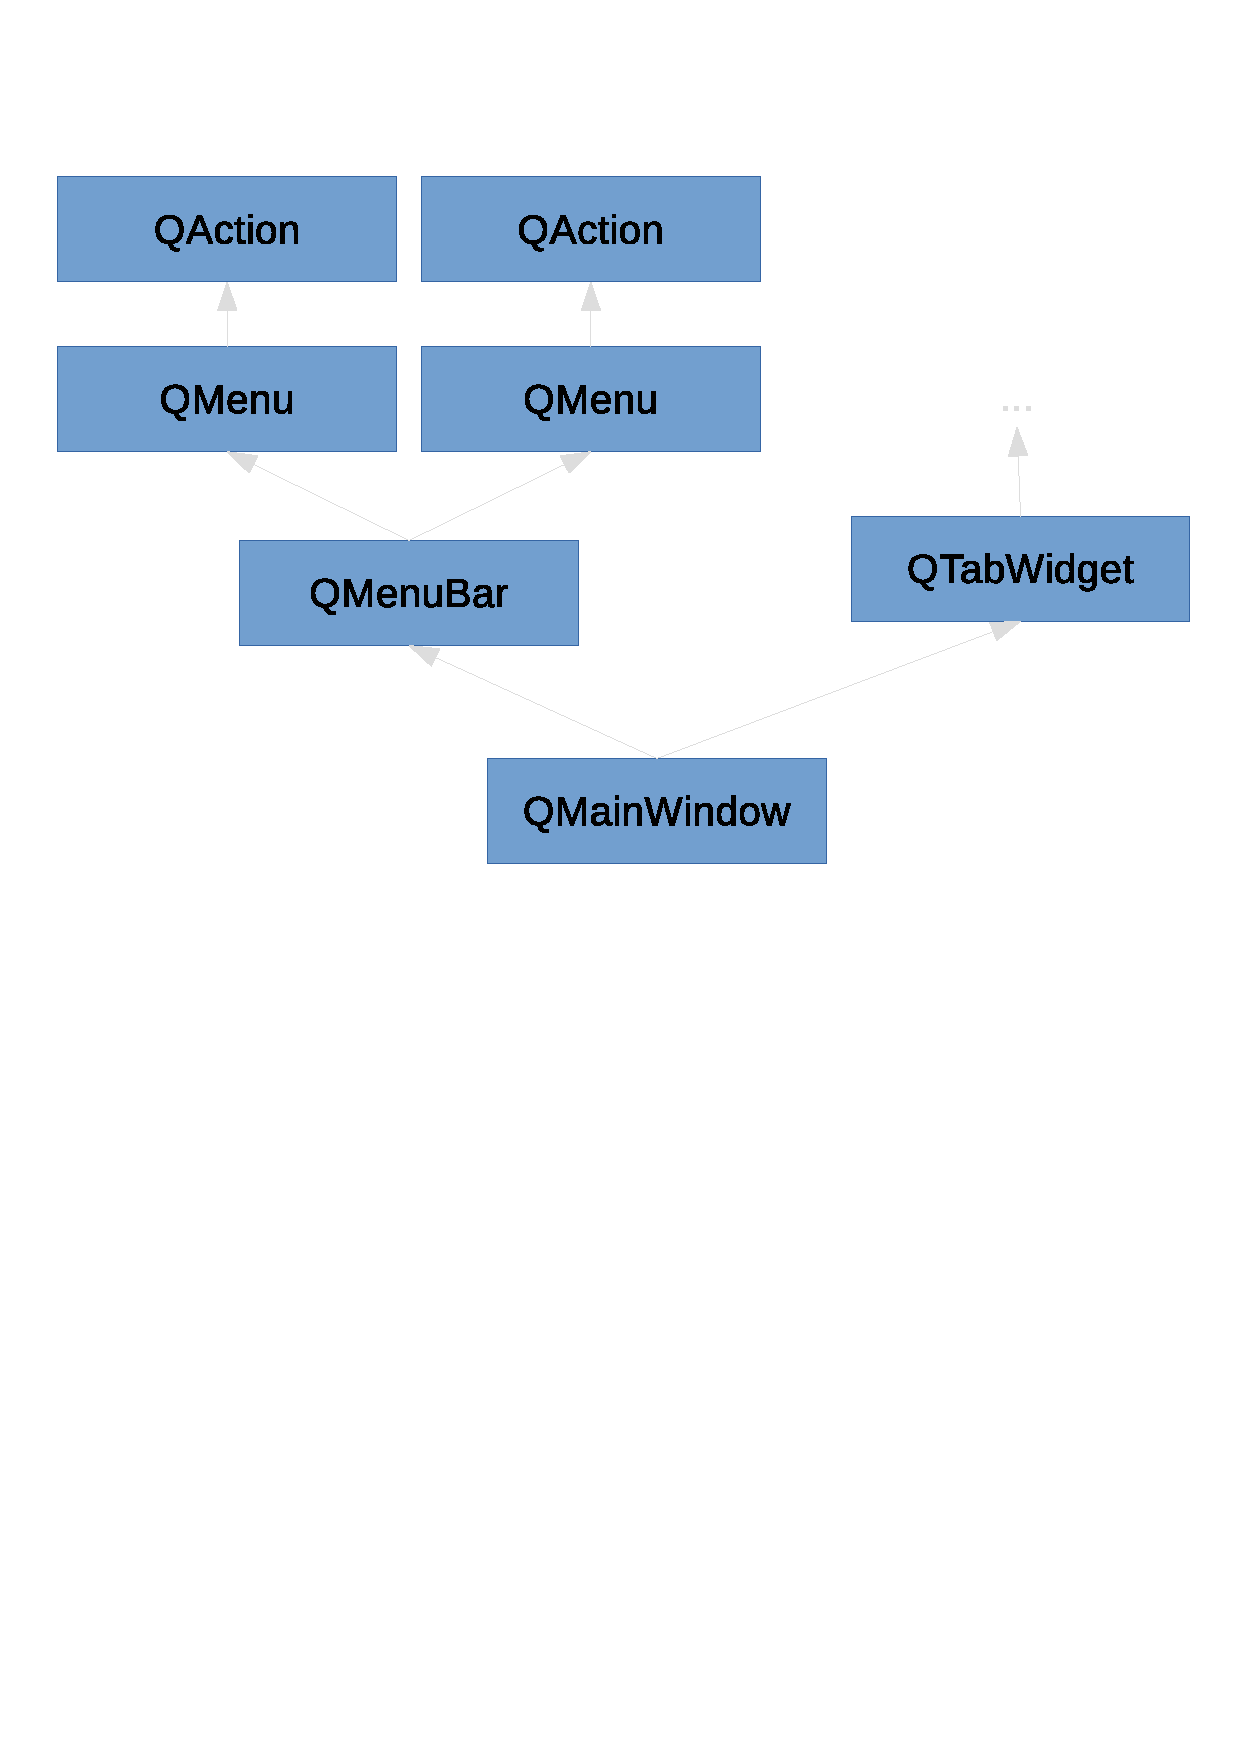
\includegraphics[scale=0.5]{hierarchy}
\end{frame}

\begin{frame}
  \frametitle{QVariant}

  QVariant is a sum of all plain types : string + int + bool + \ldots

  It is mapped to a simple OCaml variant.

  Useful to specify data models (more on that later).
\end{frame}

\subsection{Control flow}

\begin{frame}
  \frametitle{Mapping Qt concepts to OCaml}

  Qt concepts affecting control-flow:
  \begin{itemize}
    \item methods \& functions
    \item signals \& slots
    \item models
  \end{itemize}
\end{frame}

\begin{frame}[fragile]
  \frametitle{Methods \& functions}

  Methods (including static methods) are mapped to simple OCaml functions.
  They are put in a module named after the class:

  \begin{lstlisting}[language=Caml,morekeywords={module,sig,end,val}]
  module QWidget : sig
    ...
    val show : [> qWidget] qt -> unit
    val hide : [> qWidget] qt -> unit
    ...
  end 
  \end{lstlisting}

\end{frame}

\begin{frame}[fragile]
  \frametitle{Constructors}

  Constructors are very similar but they are defined in the top module and the
  naming differs a bit: 

  \begin{lstlisting}[language=Caml,morekeywords={module,sig,end}]
  val new'QPushButton : unit -> qPushButton qt
  \end{lstlisting}

\end{frame}

\begin{frame}[fragile]
  \frametitle{Working around overloading}

  Qt uses and abuses overloading.
  Imported functions are disambiguised automatically:

  \begin{lstlisting}[language=Caml,morekeywords={module,sig,end,val}]
  val setFormat : string -> ...
  val setFormat'1 : QColor -> ...
  val setFormat'2 : QFont -> ...
  \end{lstlisting}

  A {\bf curation} work is needed, to remove some variant or pick better names.
\end{frame}

\begin{frame}
  \frametitle{Signals and slots}

  The main primitive for dynamic control flow:

  \begin{itemize}
    \item a descendant of QObject can define signals and slots
    \item a {\bf signal} can be connected to {\bf slots} and {\bf closures}
    \item a signal can be emitted
    \item the slots and closures that are connected are notified
  \end{itemize}
\end{frame}

\begin{frame}[fragile]
  \frametitle{Signals and slots}

\begin{lstlisting}[language=Caml,morekeywords={module,sig,end,val}]
type (-'a, +'b) signal
type (-'a, -'b) slot

val connect_slot :  'a t -> ('a, 't) signal 
                 -> 'b t -> ('b, 't) slot -> unit

val connect :  'a t -> ('a, 't) signal 
            -> ('t -> unit) -> unit
\end{lstlisting}

\end{frame}

\begin{frame}[fragile]
  \frametitle{Signals and slots}

\begin{lstlisting}[language=Caml,morekeywords={module,sig,end,val}]
connect_slot button1 (QButton.signal'clicked())
             action1 (QAction.slot'trigger());

connect action1 (QAction.slot'triggered())
  (fun _ -> print_endline "Action!");
\end{lstlisting}

  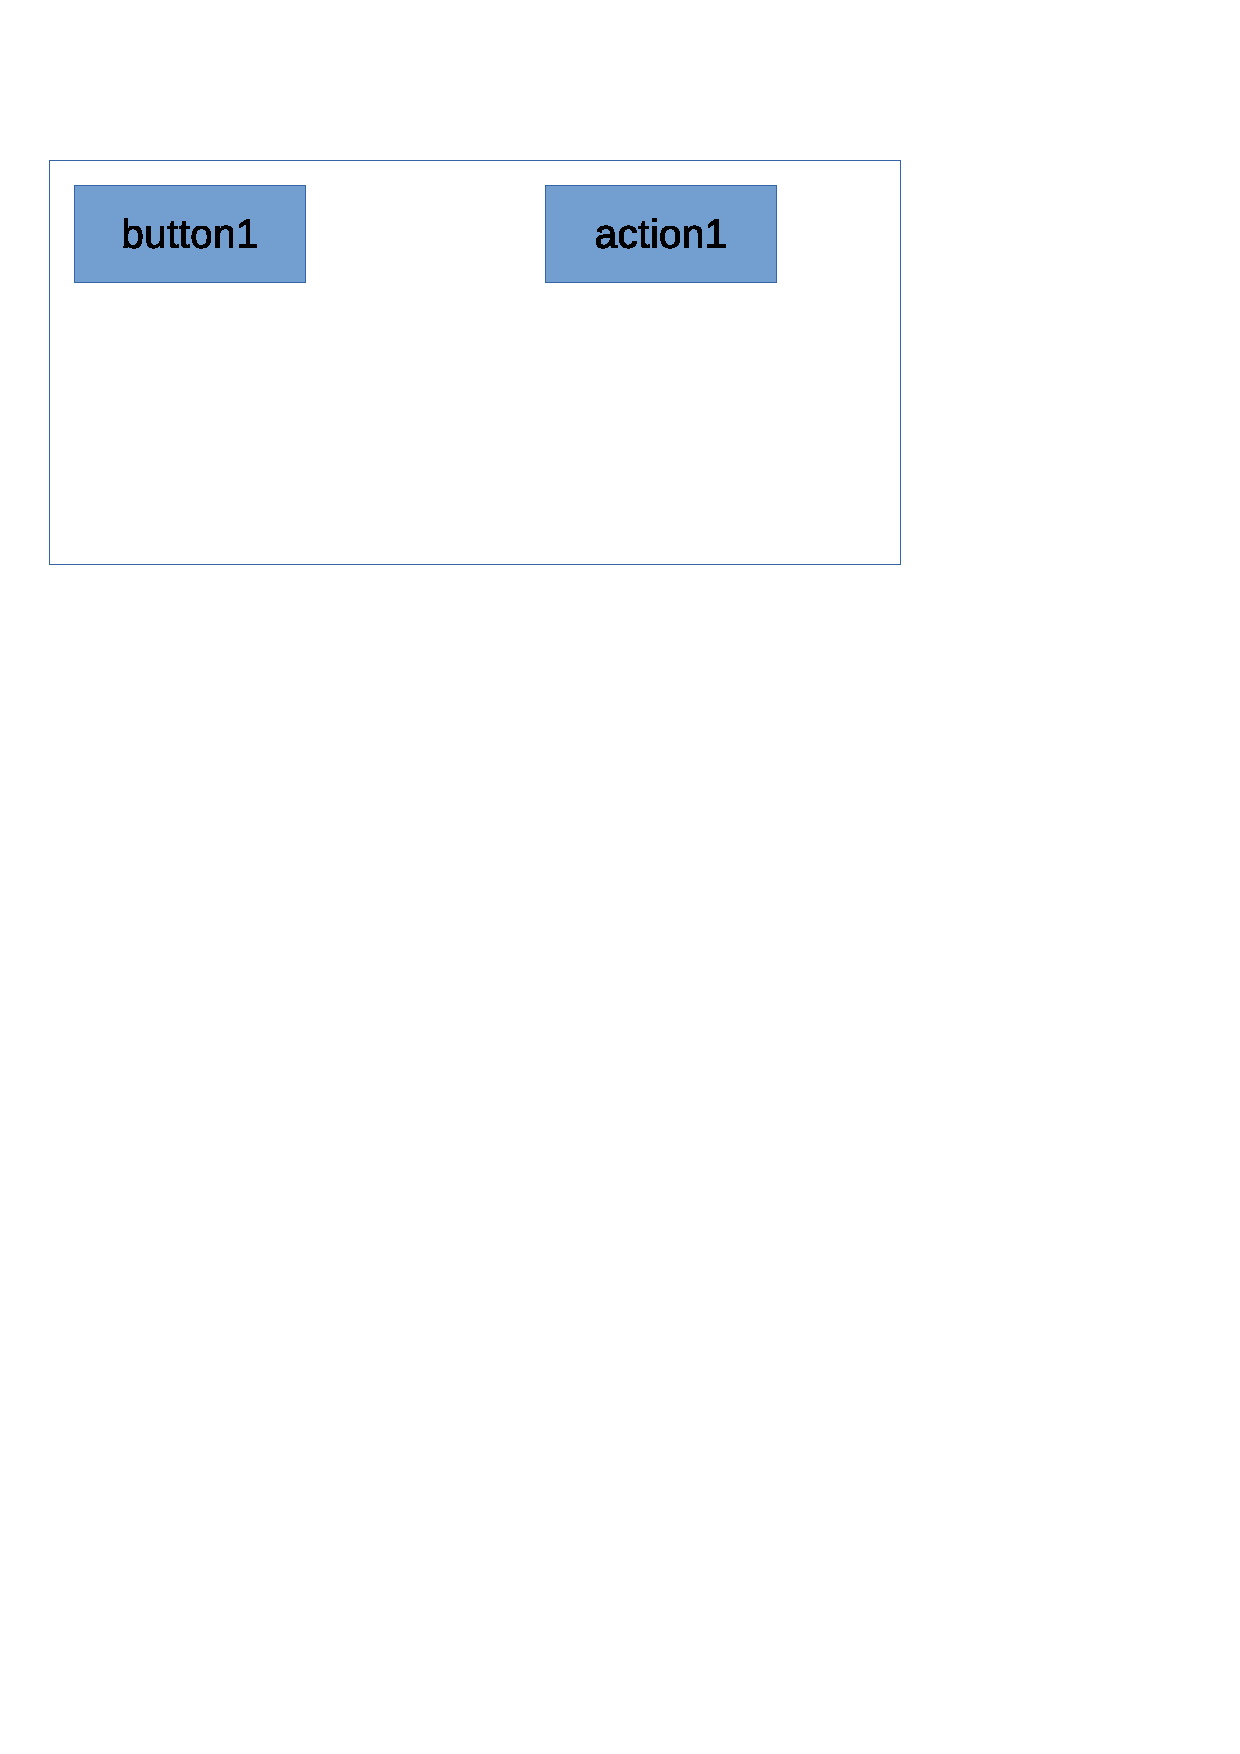
\includegraphics[scale=0.5]{slot_graph_1}

\end{frame}


\begin{frame}[fragile]
  \frametitle{Signals and slots}

\begin{lstlisting}[language=Caml,morekeywords={module,sig,end,val}]
connect_slot button1 (QButton.signal'clicked())
             action1 (QAction.slot'trigger());

connect action1 (QAction.slot'triggered())
  (fun _ -> print_endline "Action!");
\end{lstlisting}

  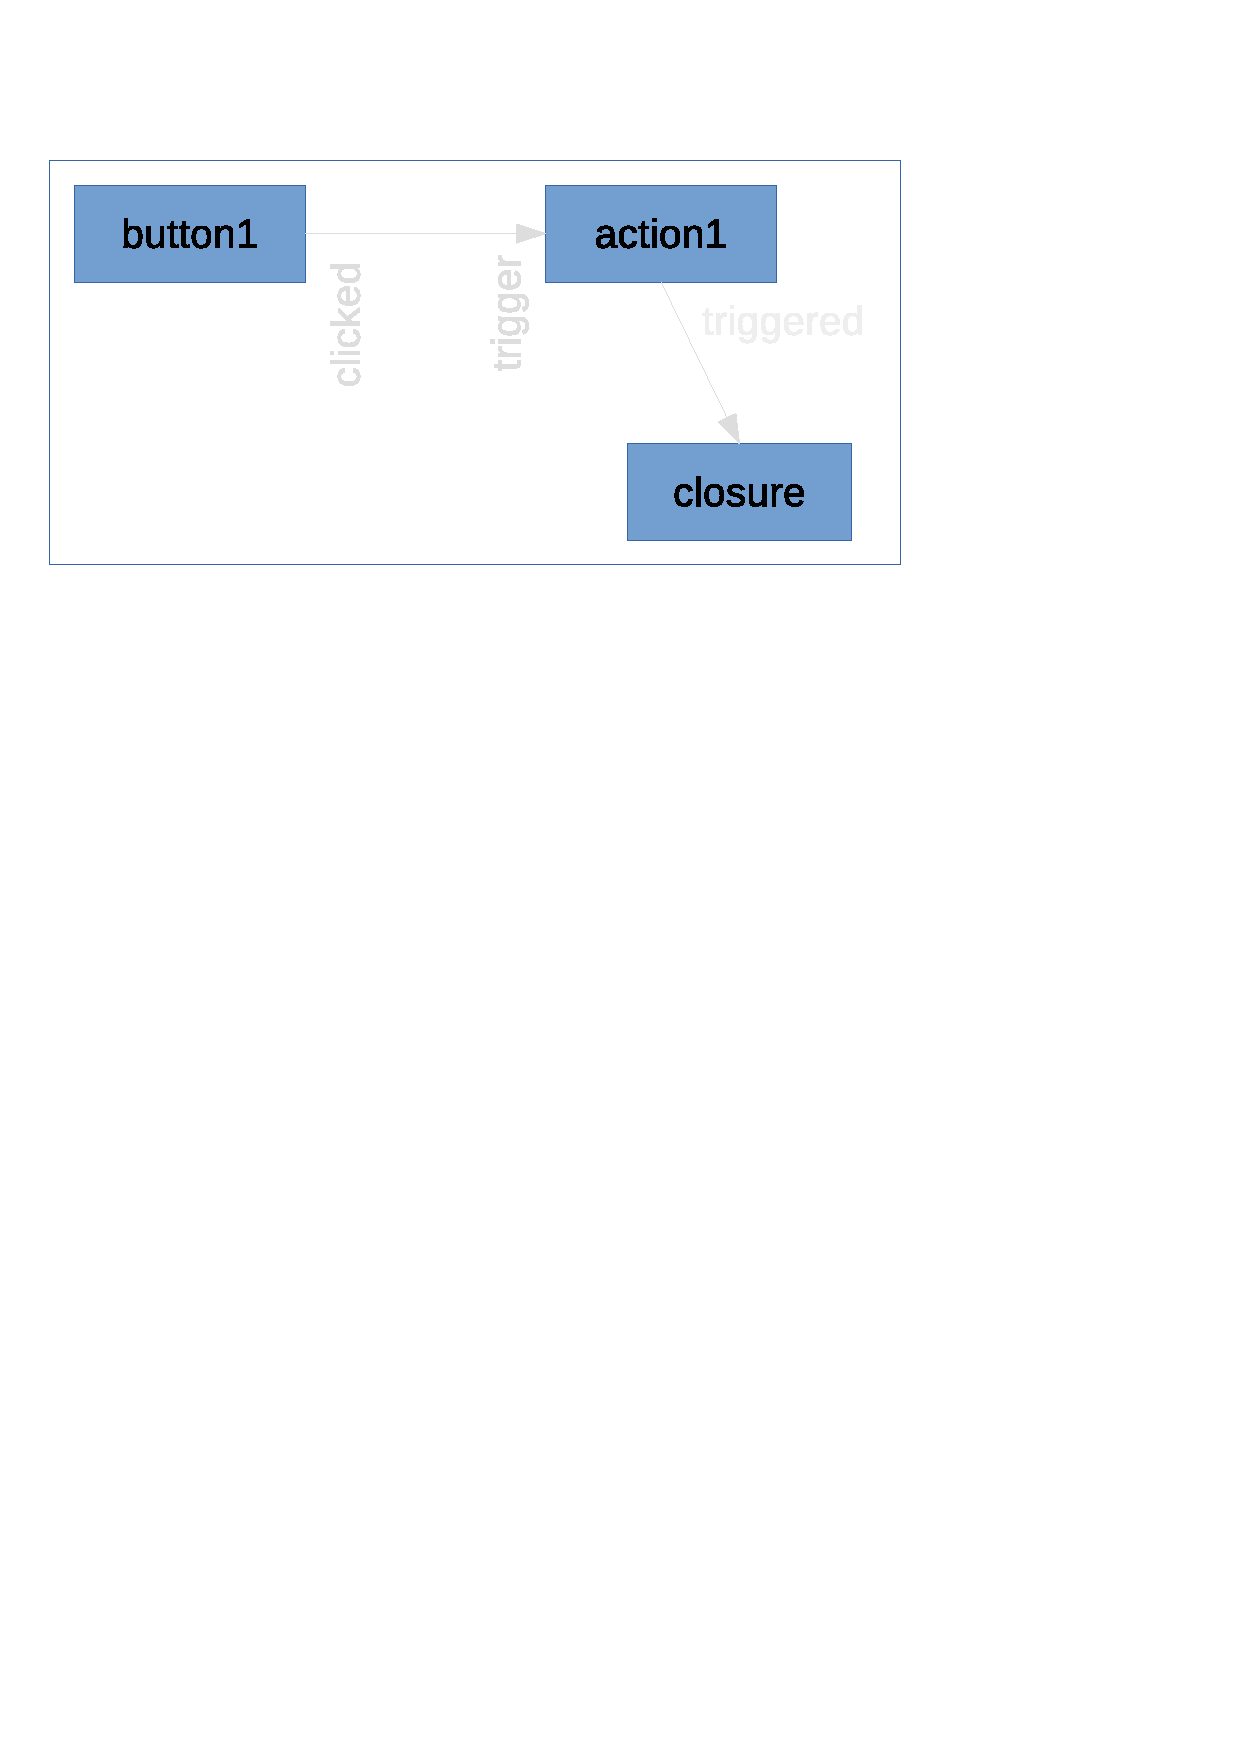
\includegraphics[scale=0.5]{slot_graph_2}

\end{frame}


\begin{frame}
  \frametitle{Models}

  Models are used to specify dynamic {\bf data source}.

  \medskip

  An abstract model is a QObject with one or more virtual methods that define
  {\bf observations on a set of data}:

  \begin{itemize}
    \item how many items
    \item content or display properties of each item
    \item structure of the items: tree-like, tabular, etc
  \end{itemize}

\end{frame}

\begin{frame}
  \frametitle{Models}

  Each Model has to be encoded manually in OCaml.

  The encoding is in two parts:

  \begin{itemize}
    \item the class is inherited only once on C++ side
    \item an instance wraps an OCaml record that contains a closure for each method
  \end{itemize}

  No C++ has to be written by the user :).

\end{frame}


\begin{frame}
  \frametitle{Models}

  Example: 
  \begin{itemize}
    \item QOCamlTableModel
    \item QOCamlSyntaxHighlighter
  \end{itemize}

\end{frame}

\subsection{Memory management}

\begin{frame}
  \frametitle{Managing QObject}
  
  Four cases for memory management:

  \begin{itemize}
    \item {\bf Relocatable objects} (plain types not mapped to a native OCaml type).  Safe, automatic, don't affect graph. \pause
    \item {\bf QObject}.
      Safe, automatic, one region released at a time. \pause
    \item {\bf Scarce resources} (e.g sockets, GPU buffers\ldots).
      Safe, manual management but GC can catch mistakes. \pause
    \item {\bf Raw pointers} (e.g. iterators).
      Unsafe, manually managed, should ideally be hidden behind an OCaml-ish
      abstraction \pause
  \end{itemize}

  Convenience/performance trade-off: when possible, release manually.
\end{frame}

\begin{frame}[fragile]
  \frametitle{Managing QObject}

  One primitive for all objects :
  
\begin{lstlisting}[language=Caml,morekeywords={module,sig,end,val}]
val delete : _ qt -> unit
\end{lstlisting}

  \begin{itemize}
    \item release Object memory
    \item for QObject, also releases all children
    \item detect use after free
    \item but cannot track aliasing of raw pointers :-(
  \end{itemize}

\end{frame}

\section{In practice}

\begin{frame}[fragile]
  \frametitle{Getting started}

  Install qt5 and cuite package.

\begin{lstlisting}[]
# yaourt -S qt5
# opam pin add cuite 
    https://github.com/let-def/cuite.git
\end{lstlisting}

\pause
  Portability not a concern yet:

  \begin{itemize}
    \item tested only with {\bf Qt 5.9}
    \item rely on {\bf pkg-config} for finding Qt5
    \item rely on {\bf g++} for compilation
    \item rely on {\bf -rpath} linker option for finding dynamic libraries
  \end{itemize}
\end{frame}

\begin{frame}[fragile]
  \frametitle{Minimal example}

  \begin{lstlisting}[language=Caml,morekeywords={module,sig,end,val,new,open}]
open Cuite

let () =
  let app = new'QApplication Sys.argv in
  let window = new'QMainWindow None QFlags.empty in
  let button = new'QPushButton'1 "Close me" None in
  QMainWindow.setCentralWidget window button;
  Qt.connect_slot'
    button (QPushButton.signal'clicked1())
    app (Qt.slot_ignore(QApplication.slot'quit()));
  QWidget.show window;
  exit (QApplication.exec ())

# ocamlfind opt -linkpkg -package cuite -o test test.ml
  \end{lstlisting}

\end{frame}

\section{Workflow and future development}

\begin{frame}
  \frametitle{Approach}

  \begin{itemize}
    \item Manually map primitive concepts (objects, classes, methods, signals,
      slots, variants, \ldots)
      \pause
    \item Automatically generate compositions of these concepts (taking an
      abstract description of Qt has OCaml values)
      \pause
    \item Manually handle corner cases (e.g models)
  \end{itemize}

\end{frame}

\begin{frame}
  \frametitle{Automatic generation}

  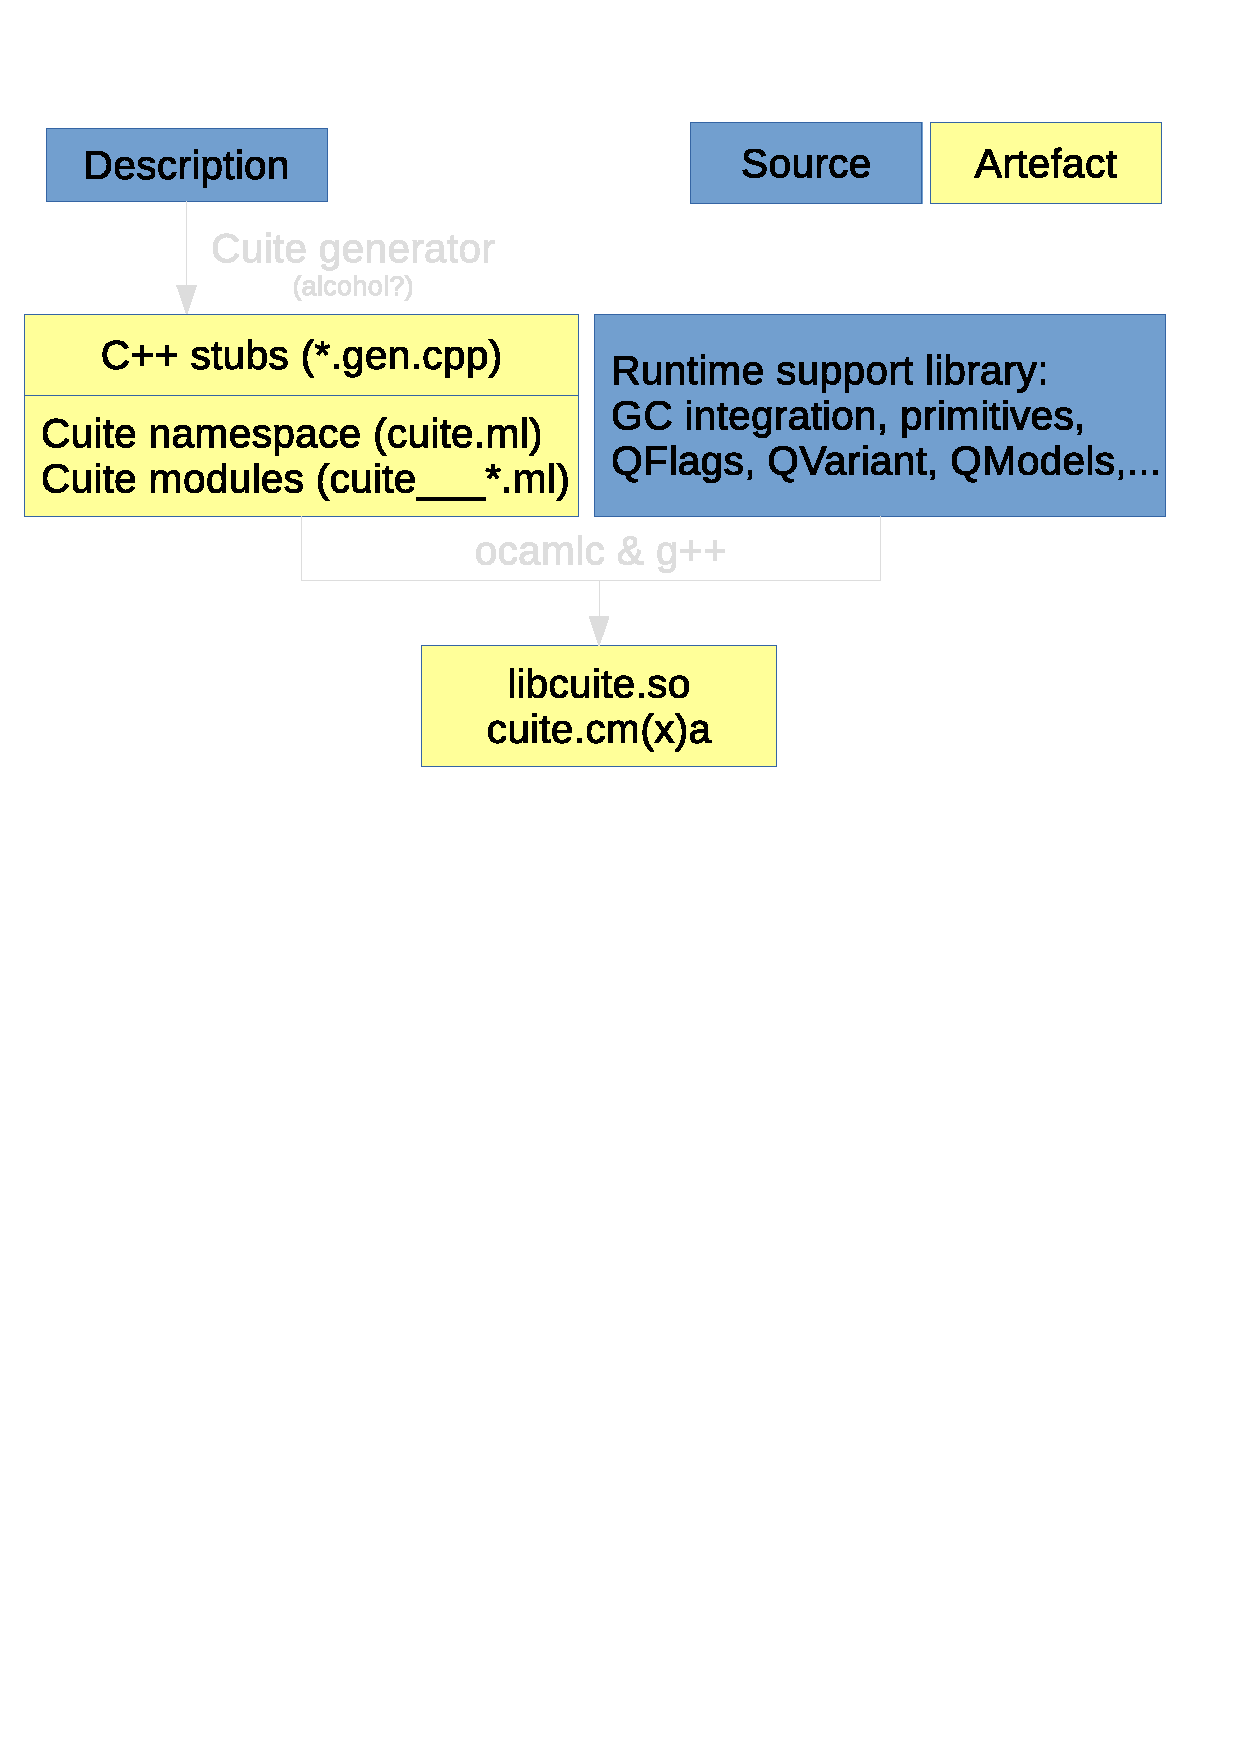
\includegraphics[width=\textwidth]{compilation_workflow}

\end{frame}

\begin{frame}
  \frametitle{Future work}

  A "proof-of-concept" has been made for each of these concepts.
  \pause

  The majority of Qt Gui/Widgets library is available\ldots but a few crucial
  parts are still missing.
  \pause

  Never ending work: too much to be handled alone, better to fix/extend as new
  use cases present themselves. 
\end{frame}

\begin{frame}
  \frametitle{Future work}

  Things to investigate:
  \begin{itemize}
    \item Qt-designer support (seems "easy", a PPX could do)
    \item Lwt/Async integration
    \item targeting mobile platforms 
    \item a multi-theading story?
    \item cleaning up ad-hoc polymorphism/overloading mess
  \end{itemize}
\end{frame}

\begin{frame}
  \frametitle{Conclusion}

  Thanks for your attention!
  \bigskip
  
  Don't hesitate to ask for guidance if you are interested in making use of
  the lib or contributing.
  \bigskip

  {
    \center 

    \huge (-:
  
  }

\end{frame}

\end{document}
